\documentclass[12pt]{article}
\usepackage{pdfpages}
\usepackage{setspace}
\usepackage[dutch]{babel}

% Importeer configuratie-instellingen
\newcommand{\folder}{C:/Users/Admin/Documents/Github/Statistiek}
\RequirePackage{\folder/LaTeX/styles/exam_config}
\RequirePackage{\folder/LaTeX/styles/statistics-macros}

\renewcommand{\baselinestretch}{1.5}
% Begin van het document
\begin{document}

% FMW-specifiek titelblad voordat het examen begint

\includepdf[pages=-]{\folder/Python/FMW_titelblad_20260605.pdf}

% \title{Tentamen statistiek}
% \author{Nederlandse Defensie Academie}
% \date{\today}
% \maketitle


\includepdf[pages=-]{\folder/LaTeX/formulebladen/Formuleblad_STA1_2026.pdf}

% Include questions from external files
\begin{question}{20}{
    Tijdens een trainingsdag wordt een alarmsituatie gehouden op de Trip van Zoudtlandtkazerne.
    Van \'e\'en peloton worden de reactietijden (in seconden) gemeten tussen het afgaan van het alarm en het moment dat de militair volledig gevechtsgereed is.

    De gemeten reactietijden van de militairen in het peloton zijn als volgt:
    \[
        18,\; 21,\; 19,\; 25,\; 23,\; 22,\; 20,\; 24,\; 26,\; 19,\; 21,\; 23,\; 27,\; 30,\; 18,\; 22,\; 24,\; 35,\; 28,\; 20.
    \]
}
        \subquestion{10}{
            Teken een boxplot van de reactietijden.
            Schrijf hierbij de stappen op die je hebt uitgevoerd om de vijf getallen voor de boxplot te kunnen bepalen.
        }
        \solution{
            Om de vijf getallen voor de boxplot te bepalen, volgen we de volgende stappen:
            \begin{itemize}
                \item Sorteer de gegevens van laag naar hoog:
                \[
                    18,\; 18,\; 19,\; 19,\; 20,\; 20,\; 21,\; 21,\; 22,\; 22,\; 23,\; 23,\; 24,\; 24,\; 25,\; 26,\; 27,\; 28,\; 30,\; 35. \rubric{1}
                \] 
                \item De minimumwaarde is $18$ en de maximumwaarde is $35$.\rubric{1}
                \item Aangezien het aantal waarden $n = 20$, dus $n$ is even, is de mediaan (tweede kwartiel) het gemiddelde van de twee middelste waarden: $\frac{22 + 23}{2} = 22.5$.\rubric{1}
                \item Het eerste kwartiel $Q_1$ is de mediaan van de laagste \SI{50}{\percent} waarden ($18, 18, 19, 19, 20, 20, 21, 21, 22, 22$).
                Aangezien er $10$ waarden zijn, is het eerste kwartiel het gemiddelde van de vijfde en zesde waarde: $Q_1=\frac{20 + 20}{2} = 20$.\rubric{2}
                \item Het derde kwartiel $Q_3$ is de mediaan van de laagste \SI{50}{\percent} waarden ($23, 23, 24, 24, 25, 26, 27, 28, 30, 35$).
                Aangezien er $10$ waarden zijn, is het derde kwartiel het gemiddelde van de vijfde en zesde waarde: $Q_3=\frac{25 + 26}{2} = 25.5$.\rubric{1}
            \end{itemize}
            De vijf getallen voor de boxplot zijn dus:
            \[
                \text{Minimum} = 18, \quad Q_1 = 20, \quad \text{Mediaan} = 22.5, \quad Q_3 = 25.5, \quad \text{Maximum} = 35. 
            \]
            
            We tekenen de boxplot met snorharen van $Q_1 - 1.5 \times \IQR$ tot $Q_3 + 1.5 \times \IQR$, waarbij $\IQR = Q_3 - Q_1 = 25.5 - 20 = 5.5$. \rubric{1}
            De \enquote{whiskers} lopen van de kleinste niet-outlier boven $20 - 1.5 \times 5.5 = 11.75$ (oftewel $18$) tot de hoogste niet-outlier onder $25.5 + 1.5 \times 5.5 = 33.75$ (oftewel $30$).
            Er is één outlier, namelijk $35$. \rubric{1}
            \begin{center}
                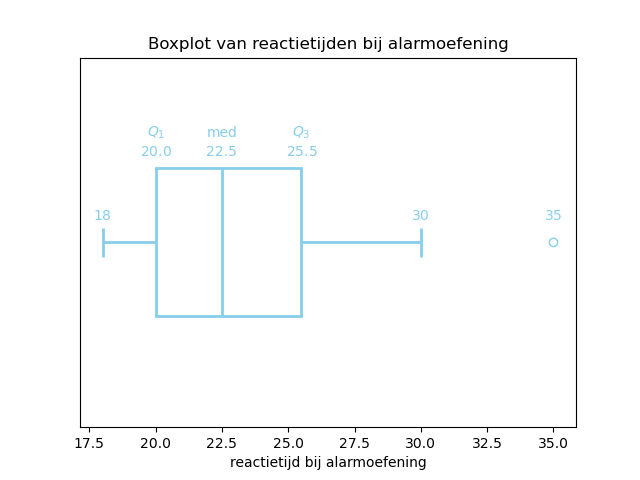
\includegraphics[width=\textwidth]{./20260605_exam_boxplot.png} \rubric{2}
            \end{center}

        }

        \subquestion{3}{
            Leg met behulp van de boxplot uit wat je kunt zeggen over de ligging van het gemiddelde ten opzichte van de mediaan?
        }
        \solution{
            Aan de boxplot is te zien dat de data een positieve scheefheid vertoont.\rubric{1}
            Dit is te zien aan de langere snorhaar aan de rechterkant van de boxplot en de aanwezigheid van een outlier aan de rechterkant.
            In een positief scheve verdeling ligt het gemiddelde hoger dan de mediaan, omdat het gemiddelde wordt beïnvloed door de hogere waarden (zoals de outlier $35$).\rubric{1}
            Daarom kunnen we concluderen dat het gemiddelde van de reactietijden hoger ligt dan de mediaan van $22.5$ seconden. \rubric{1}
        }
        \subquestion{2}{
            Noem \'e\'en reden waarom deze steekproef mogelijk niet representatief is voor de reactietijden van alle militairen in de Trip van Zoudtlandtkazerne.
        }
        \solution{
            Een mogelijke reden waarom deze steekproef niet representatief is, is dat de reactietijden alleen zijn gemeten van \'e\'en specifiek peloton.\rubric{1}
            De reactietijden kunnen variëren tussen verschillende pelotons vanwege verschillen in training, ervaring of andere factoren.
            Hierdoor zou de resultaten van deze steekproef mogelijk niet generaliseerbaar kunnen zijn naar alle militairen in de Trip van Zoudtlandtkazerne. \rubric{1}
        }

        \subquestion{5}{
            Tijdens de analyse ontdekt men dat er een fout is gemaakt bij het invoeren van de reactietijd van een van de militairen, en dat deze reactietijd eigenlijk $40$ seconden had moeten zijn in plaats van $30$ seconden. Geef aan wat er zou veranderen aan de boxplot als deze fout wordt gecorrigeerd.
        }
        \solution{
            Als de fout wordt gecorrigeerd en de reactietijd van $30$ seconden wordt vervangen door $40$ seconden, zal dit de maximumwaarde in de dataset veranderen van $35$ naar $40$.\rubric{1}
            De minimumwaarde, het eerste kwartiel, de mediaan en het derde kwartiel zullen echter niet veranderen, omdat deze waarden niet worden beïnvloed door de hoogste waarde in de dataset.\rubric{2}
            De whisker aan de rechterkant van de boxplot zal nu lopen tot de hoogste niet-outlier onder $25.5 + 1.5 \times 5.5 = 33.75$, oftewel $28$, en er zullen nu twee outliers zijn: $35$ en $40$. \rubric{2}
            \begin{center}
                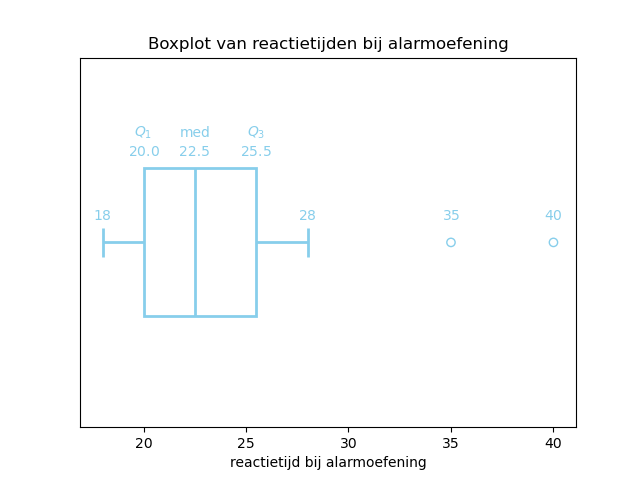
\includegraphics[width=\textwidth]{./20260605_exam_boxplot2.png}
            \end{center}
        }
\end{question}
\begin{question}{25}{
    a
}
    \subquestion{10}{
        
    }
    \solution{
        
    }
\end{question}
\begin{question}{25}{
    De Westelijke Balkanroute is een belangrijke migratieroute richting de Europese Unie. 
    Mensensmokkelnetwerken proberen migranten clandestien vanuit Bosnië en Herzegovina de grens over te loodsen naar EU-lidstaat Kroatië. 
    De Koninklijke Marechaussee (KMar) ondersteunt de Kroatische grenspolitie met geavanceerde thermische bewakingscamera's en mobiele sensorsystemen. 
    
    De tijd $X$ (in minuten) die het sensorsysteem van de KMar nodig heeft voor initiële detectie en beeldverificatie van illegale overstekers is normaal verdeeld met gemiddelde $\mu=4.12$ minuten en een standaardafwijking $\sigma=0.76$ minuten.
}
    \subquestion{7}{
        Zodra de illegale overstekers de grens oversteken, moeten ze zorgen dat ze zo snel mogelijk aan het zicht verdwijnen van de thermische camera's door de dichte bebossing aan de Kroatische zijde te bereiken.
        De tijd $Y$ die een groep overstekers hiervoor nodig heeft is normaal verdeeld met een gemiddelde van $\mu(Y) = 5.0$ minuten en een standaardafwijking van $\sigma(Y) = 0.34$ minuten.
        Bereken de kans dat een individuele smokkelpoging \textit{succesvol} is omdat de analyse en verificatie pas voltooid zijn nadat de overstekers uit het zicht zijn verdwenen.
    }
    \solution{
        We hebben in deze situatie te maken met twee kansvariabelen $X$ en $Y$, zoals die hierboven gedefinieerd zijn.
        De kans dat een individuele smokkelpoging succesvol is, is gelijk aan de kans dat de overstekers sneller uit het zicht verdwijnen $P(X > Y)$.\rubric{1}
        Definieer hiertoe de verschilvariabele $V = X - Y$. We willen dus de kans $P(X > Y)$, oftewel $P(V = X - Y > 0)$ berekenen.\rubric{1}

        Aangezien zowel $X$ als $Y$ normaal verdeeld zijn, geldt in dit geval dat de verschilvariabele $V = X - Y$ ook normaal verdeeld is met:
        \begin{align*}
            E(V)        &= \mu(X) - \mu(Y) = 4.12 - 5.0 = -0.78 \\
            \sigma(V)   &= \sqrt{\sigma(X)^2 + \sigma(Y)^2} = \sqrt{0.76^2 + 0.34^2} \approx 0.8326 \rubric{2}
        \end{align*}

        De gevraagde kans $P(V > 0)$ berekenen we dan als volgt:
        \begin{align*}
            P(V > 0)    &= \normalcdf(\lb=0, \ub=10^{99}, \mu=-0.78, \sigma=0.8326) \\
                        &\approx 0.1744. \rubric{2}  
        \end{align*}
        De kans dat een smokkelpoging slaagt vanwege een trage reactie van het systeem, bedraagt dus \textbf{0.1744} (of \SI{17.44}{\percent}).\rubric{1}
    }

    \subquestion{7}{
        De KMar wil de effectiviteit van het grensbeheer verhogen. 
        Technici stellen voor om de processors in de sensorsystemen te vervangen door snellere AI-chips. 
        Hierdoor zal de gemiddelde verificatietijd $\mu(X)$ dalen.
        De standaardafwijking $\sigma(X)$ van de sensorsystemen en de kansverdeling van $Y$ blijven ongewijzigd.
        Bereken met hoeveel minuten de gemiddelde verificatietijd $\mu(X)$ gereduceerd moet worden zodat de kans op een succesvolle oversteek nog maar \SI{5}{\percent} is.
    }
    \solution{
        We hebben in deze situatie weer te maken met twee kansvariabelen $X$ en $Y$, maar nu is de verwachtingswaarde $\mu(X)$ een te bepalen onbekende.\rubric{1}
        Met andere woorden, de verschilvariabele $V = X - Y$ is nu normaal verdeeld met:
        \begin{align*}
            E(V)        &= \mu(X) - \mu(Y) = \mu(X) - 5.0 \\
            \sigma(V)   &= \sqrt{\sigma(X)^2 + \sigma(Y)^2} = \sqrt{0.76^2 + 0.34^2} \approx 0.8326 \rubric{1}
        \end{align*}

        Om de gevraagde $\mu(X)$ te berekenen, gebruiken we opnieuw de \enquote{numeric solver}:
        \begin{align*}
            E_1     &= \normalcdf(\lb=0, \ub=10^{99}, \mu=X-5.0, \sigma=0.8326) \\
            E_2     &\approx 0.05. \rubric{2}  
        \end{align*}
        Hieruit volgt een waarde van $X \approx 3.6305$.\rubric{1}
        Dit betekent dat de gemiddelde verificatietijd $\mu(X)$ gereduceerd moet worden met ongeveer $4.12 - 3.6305 = 0.4895$ minuten, oftewel net iets minder dan een halve minuut.\rubric{1}
        De kans dat een smokkelpoging slaagt vanwege een trage reactie van het systeem, bedraagt dus \textbf{0.1744} (of \SI{17.44}{\percent}).\rubric{1}
    }

    \subquestion{8}{
        De bevelhebber van de Kroatische grenspatrouille eist strengere maatregelen om de controle te behouden. 
        Door de inzet van extra KMar-drone-ondersteuning dalen de verificatietijden, waardoor de kans dat een groep ongedetecteerd wegglipt, afneemt naar $p = 0.05$ (\SI{5}{\percent}). 
        De operationele opvang- en detentiecapaciteit van de lokale Kroatische politiepost is echter strikt beperkt: de eenheden kunnen per nacht maximaal 2 groepen fysiek onderscheppen en administratief verwerken. Als er in één nacht \textit{meer dan 2} groepen door de mazen van de wet glippen, raakt de capaciteit op de grond overbelast en faalt de grensmissie.
        
        Bereken via een numerieke benadering (of systematisch uitproberen) hoeveel groepen ($n$) het smokkelnetwerk in één nacht maximaal kan inzetten, zodat de kans op overbelasting van de grensbewaking \textit{hoogstens} \SI{10}{\percent} is.
    }
    \solution{
        Laat $Y$ het aantal succesvol doorgeglipte groepen zijn met $Y \sim \text{Bin}(n, 0.05)$. 
        De capaciteit raakt overbelast als $Y > 2$. De harde eis is dat deze kans maximaal \SI{10}{\percent} mag zijn:\rubric{1}
        \[
            P(Y > 2) \leq 0.10 \implies P(Y \leq 2) \geq 0.90
        \]
        We schrijven de cumulatieve binomiale kans uit voor $Y \leq 2$:\rubric{1}
        \[
            P(Y \leq 2) = \binom{n}{0}(0.05)^0(0.95)^n + \binom{n}{1}(0.05)^1(0.95)^{n-1} + \binom{n}{2}(0.05)^2(0.95)^{n-2}
        \]
        Studenten moeten nu numeriek of via een tabel doorrekenen voor verschillende waarden van $n$ om de grens te bepalen:\rubric{2}
        \begin{itemize}
            \item $n = 20 \implies P(Y \leq 2) = 0.3585 + 0.3774 + 0.1887 = 0.9246 \geq 0.90$ (Veilig)
            \item $n = 21 \implies P(Y \leq 2) = 0.3406 + 0.3764 + 0.1981 = 0.9151 \geq 0.90$ (Veilig)
            \item $n = 22 \implies P(Y \leq 2) = 0.3235 + 0.3751 + 0.2073 = 0.9059 \geq 0.90$ (Veilig)
            \item $n = 23 \implies P(Y \leq 2) = 0.3074 + 0.3734 + 0.2163 = 0.8971 < 0.90$ (Onveilig)\rubric{3}
        \end{itemize}
        Het netwerk kan maximaal \textbf{22 groepen} tegelijk inzetten om de kans op een succesvolle overbelasting (het wegglippen van meer dan 2 groepen) onder de \SI{10}{\percent} te houden. Vanaf 23 groepen wordt het operationele risico voor de grensbewaking te groot.\rubric{1}
    }
\end{question}
\begin{question}{25}{
    Het Space Operations Centre (SpOC) van de NAVO bewaakt een constellatie van militaire communicatiesatellieten (MILSATCOM) die cruciale data-uplinks verzorgen voor grondtroepen in een operatiegebied. 
    Vijandelijke actoren passen regelmatig RF-jamming (radiofrequentie-storing) toe om deze uplinks tijdelijk te onderbreken.

    Uit operationele data over de afgelopen 18 maanden blijkt dat vijandelijke jamming-aanvallen gemiddeld $\lambda=3.2$ aanvallen per dag voorkomen volgens een Poissonproces.
    Elke aanval duurt gemiddeld $25$ minuten met een standaardafwijking van $3.5$ minuten, en verstoort de communicatieverbinding volledig voor de duur van de aanval. 

    Het SpOC beschikt over een Counter-Space Response Team (CSRT) dat actief tegenmaatregelen kan inzetten (frequentiehoppen, uplink-switching).
    Het team kan per dag maximaal $5$ aanvallen effectief neutraliseren. 
    Aanvallen boven deze capaciteit leiden tot een communicatieblackout voor de grondtroepen.
}
    \subquestion{5}{
        Bereken de kans dat het SpOC in een willekeurige week \emph{minimaal} $20$ jamming-aanvallen registreert.
    }
    \solution{
        
    }

    \subquestion{5}{
        Bereken de kans dat het CSRT op een willekeurige dag overbelast raakt. 
    }
    \solution{
        
    }

    \subquestion{5}{
        De NAVO-norm stelt dat de kans op een communicatieblackout per etmaal kleiner dan \SI{5}{\percent} moet zijn. 
        Bepaal de minimale CSRT-capaciteit (in aantallen aanvallen per dag die geneutraliseerd kunnen worden) waarmee aan deze norm wordt voldaan.
    }
    \solution{

    }

    \subquestion{}

\end{question}

% Add more question files as needed
\end{document}